\documentclass{article}
\usepackage{amsmath}
\usepackage{amssymb}
\usepackage{parallel}
\usepackage[most]{tcolorbox}
\usepackage{amsthm}
\usepackage{caption}
\usepackage{subcaption}
\usepackage[a4paper,
top=1.5cm,
bottom=1.5cm,
left=1.8cm,
right=1.8cm,
heightrounded]
{geometry}
\renewcommand{\arraystretch}{2.5}

\begin{document}
\section*{Part II: (Swaption Calibration)}
\section{Model Calibration}

\begin{figure}[h]
	\centering
	\begin{subfigure}{.5\textwidth}
		\centering
		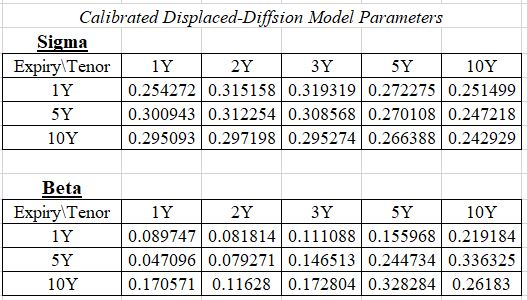
\includegraphics[width=1\linewidth]{./images/DD.jpg}
		\caption{Displaced-Diffsion Model}
		\label{fig:sub1}
	\end{subfigure}%
	\begin{subfigure}{.5\textwidth}
		\centering
		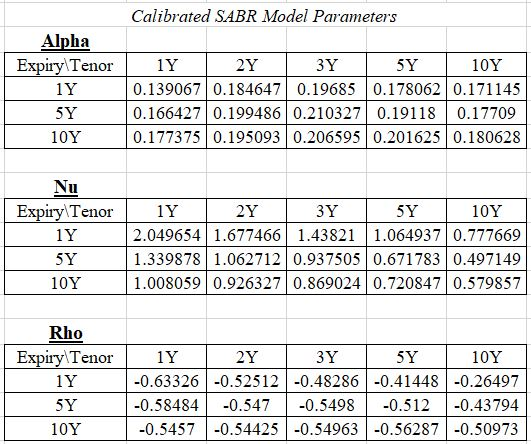
\includegraphics[width=0.7\linewidth]{./images/SABR.jpg}
		\caption{SABR Model}
		\label{fig:sub2}
	\end{subfigure}
	\caption{Parameter Calibration}
	\label{fig:test}
\end{figure}

\section{Pricing swaptions using the calibrated model}
\begin{figure}[h]
	\centering
	\begin{subfigure}{.5\textwidth}
		\centering
		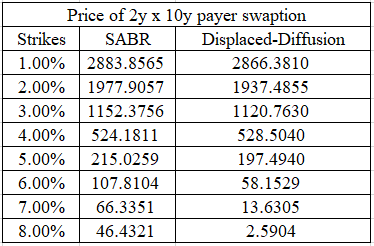
\includegraphics[width=0.9\linewidth]{./images/Payer.png}
		\caption{payer 2y x 10y}
		\label{fig:sub1}
	\end{subfigure}%
	\begin{subfigure}{.5\textwidth}
		\centering
		\includegraphics[width=0.91\linewidth]{./images/Receiver.png}
		\caption{receiver 8y x 10y}
		\label{fig:sub2}
	\end{subfigure}
	\caption{Swaption price}
	\label{fig:test}
\end{figure}

bla bla bla bla...

bla bla bla bla...

bla bla bla bla...

\newpage
\section{Fitting curve}
\begin{figure}[h]
    \flushleft
	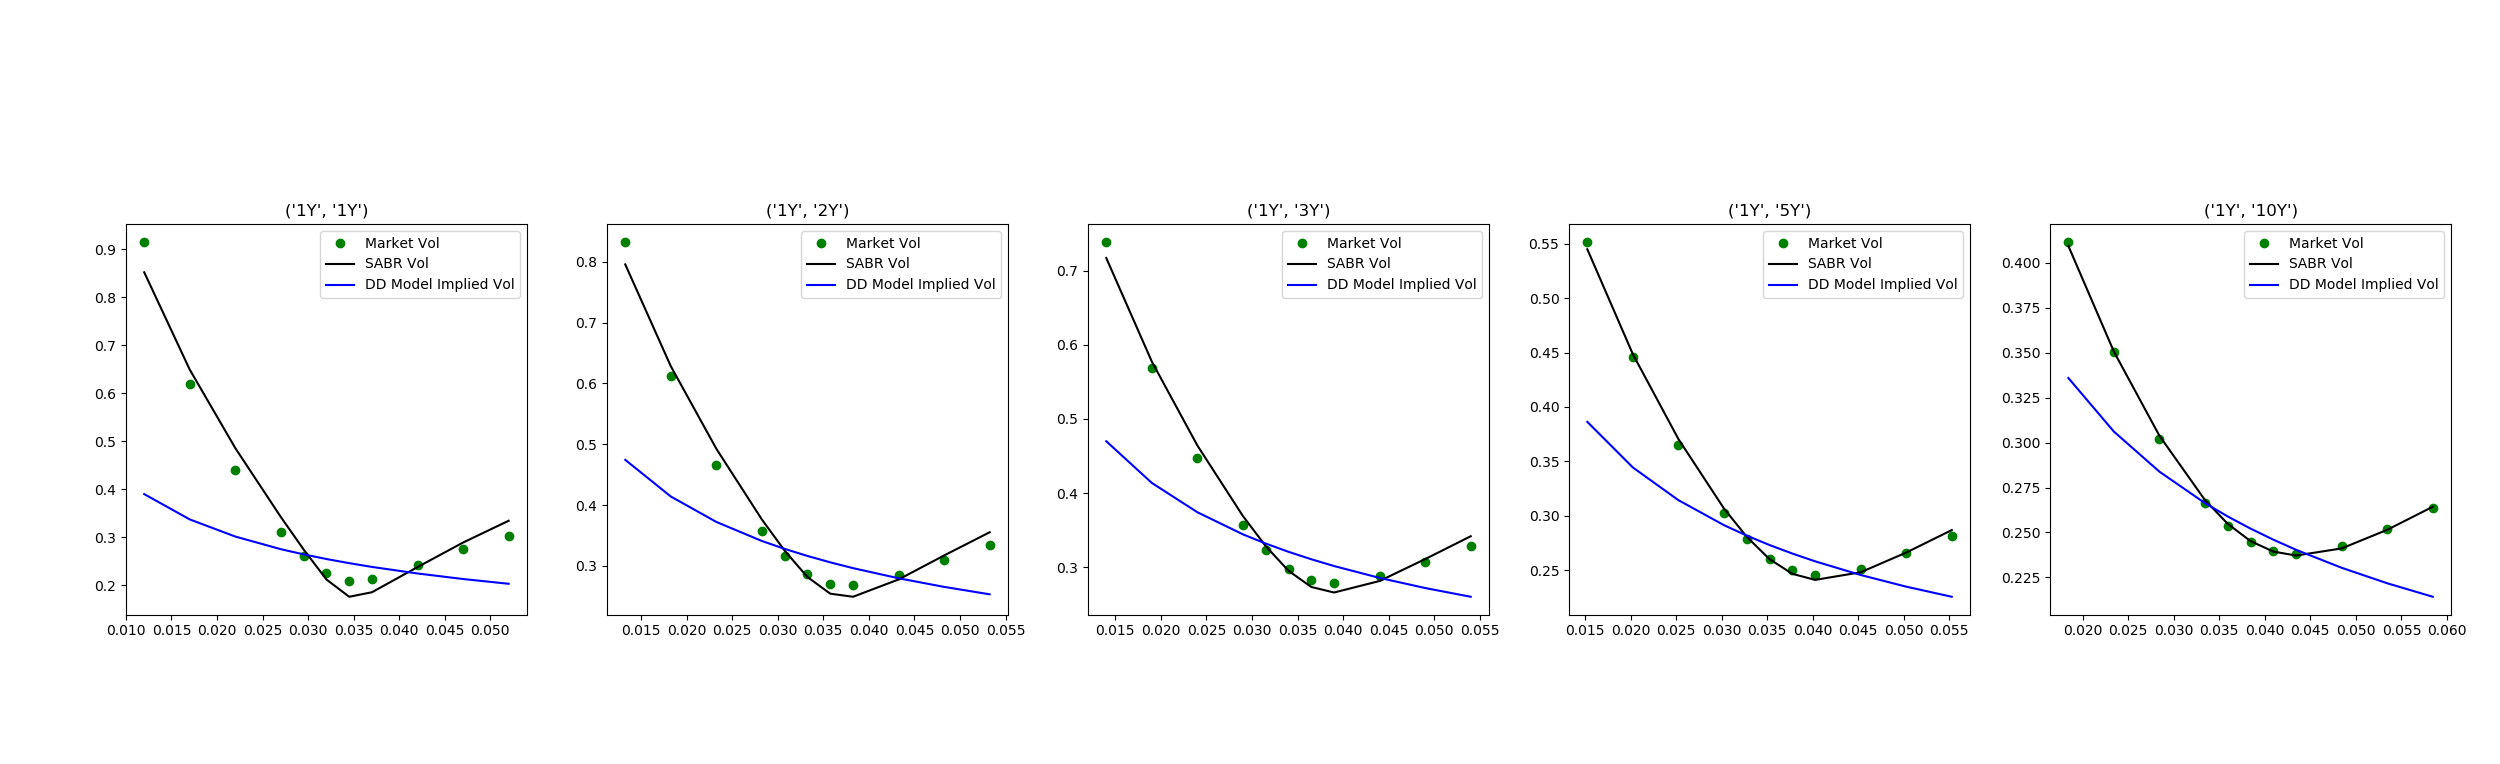
\includegraphics[width=1\linewidth]{./images/1Y.png}
	\caption{1y expiry swaption: Tenor from 1y to 10y}
	\label{fig:sub1}
\end{figure}
\begin{figure}[h]
	\flushleft
	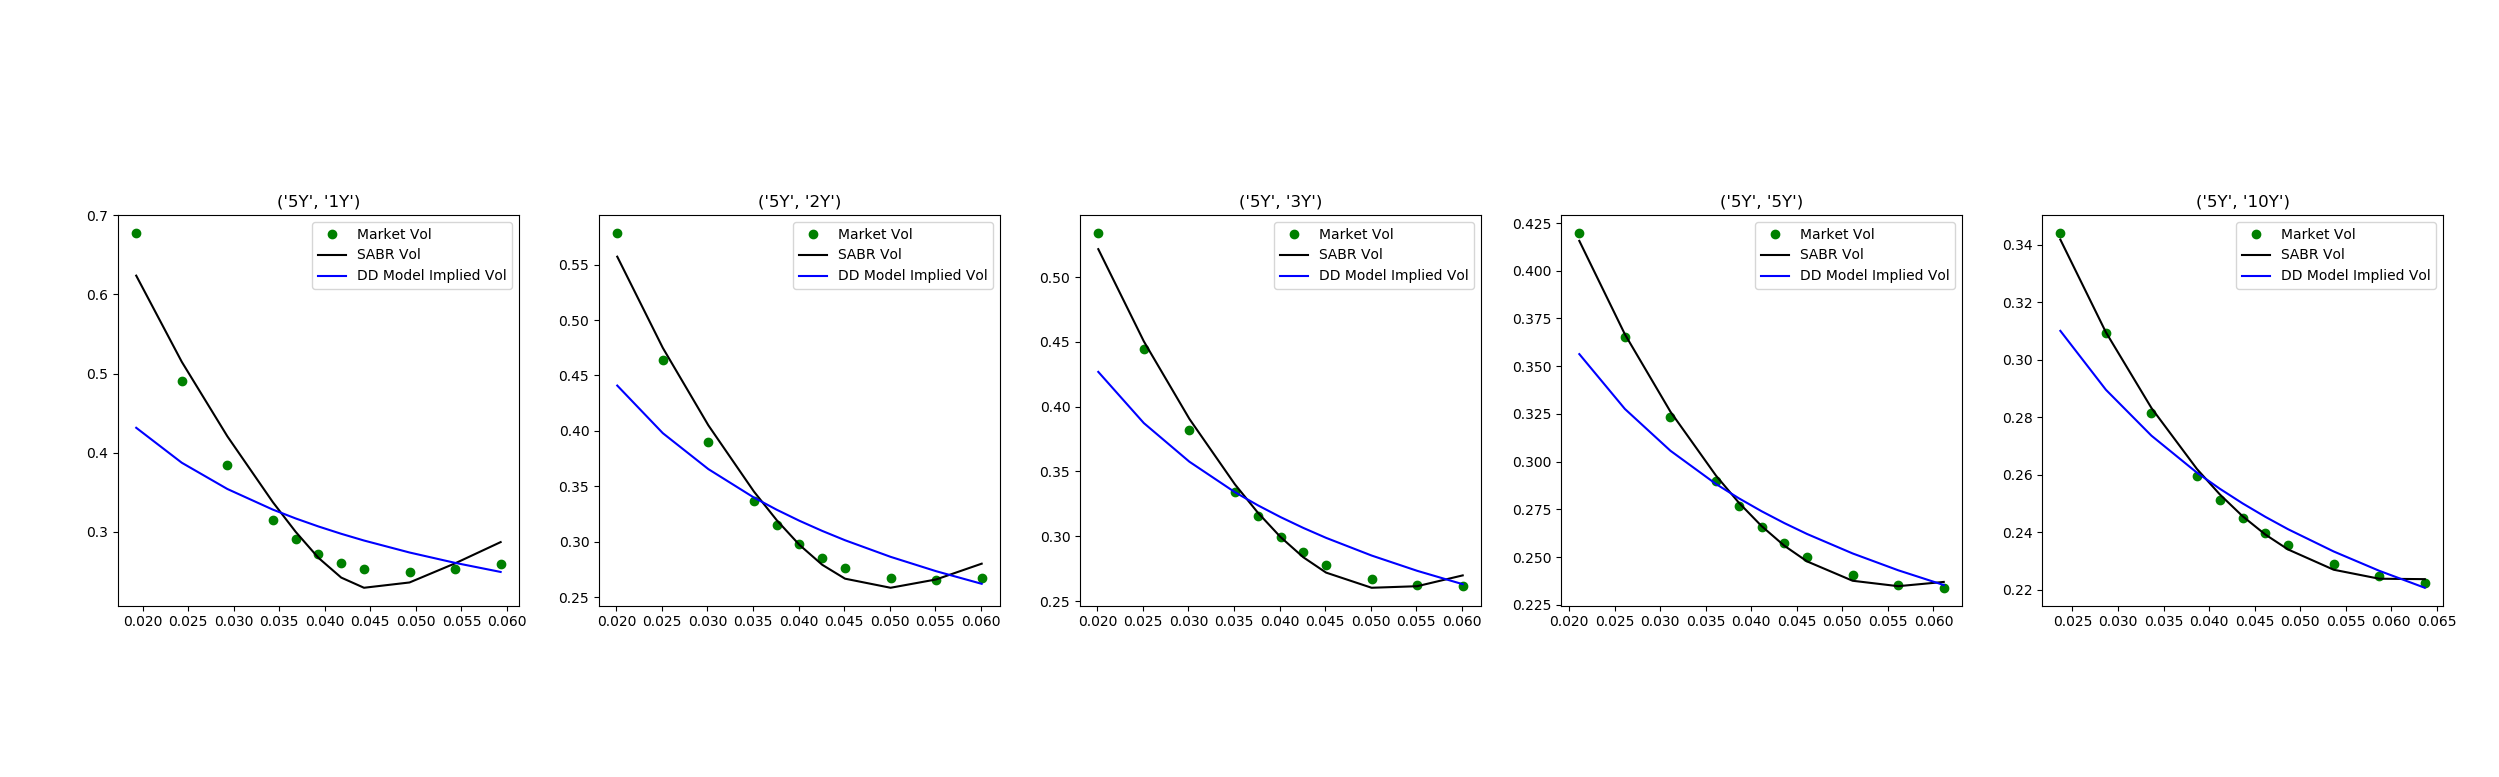
\includegraphics[width=1\linewidth]{./images/5Y.png}
	\caption{5y expiry swaption: Tenor from 1y to 10y}
	\label{fig:sub1}
\end{figure}
\begin{figure}[h]
	\flushleft
	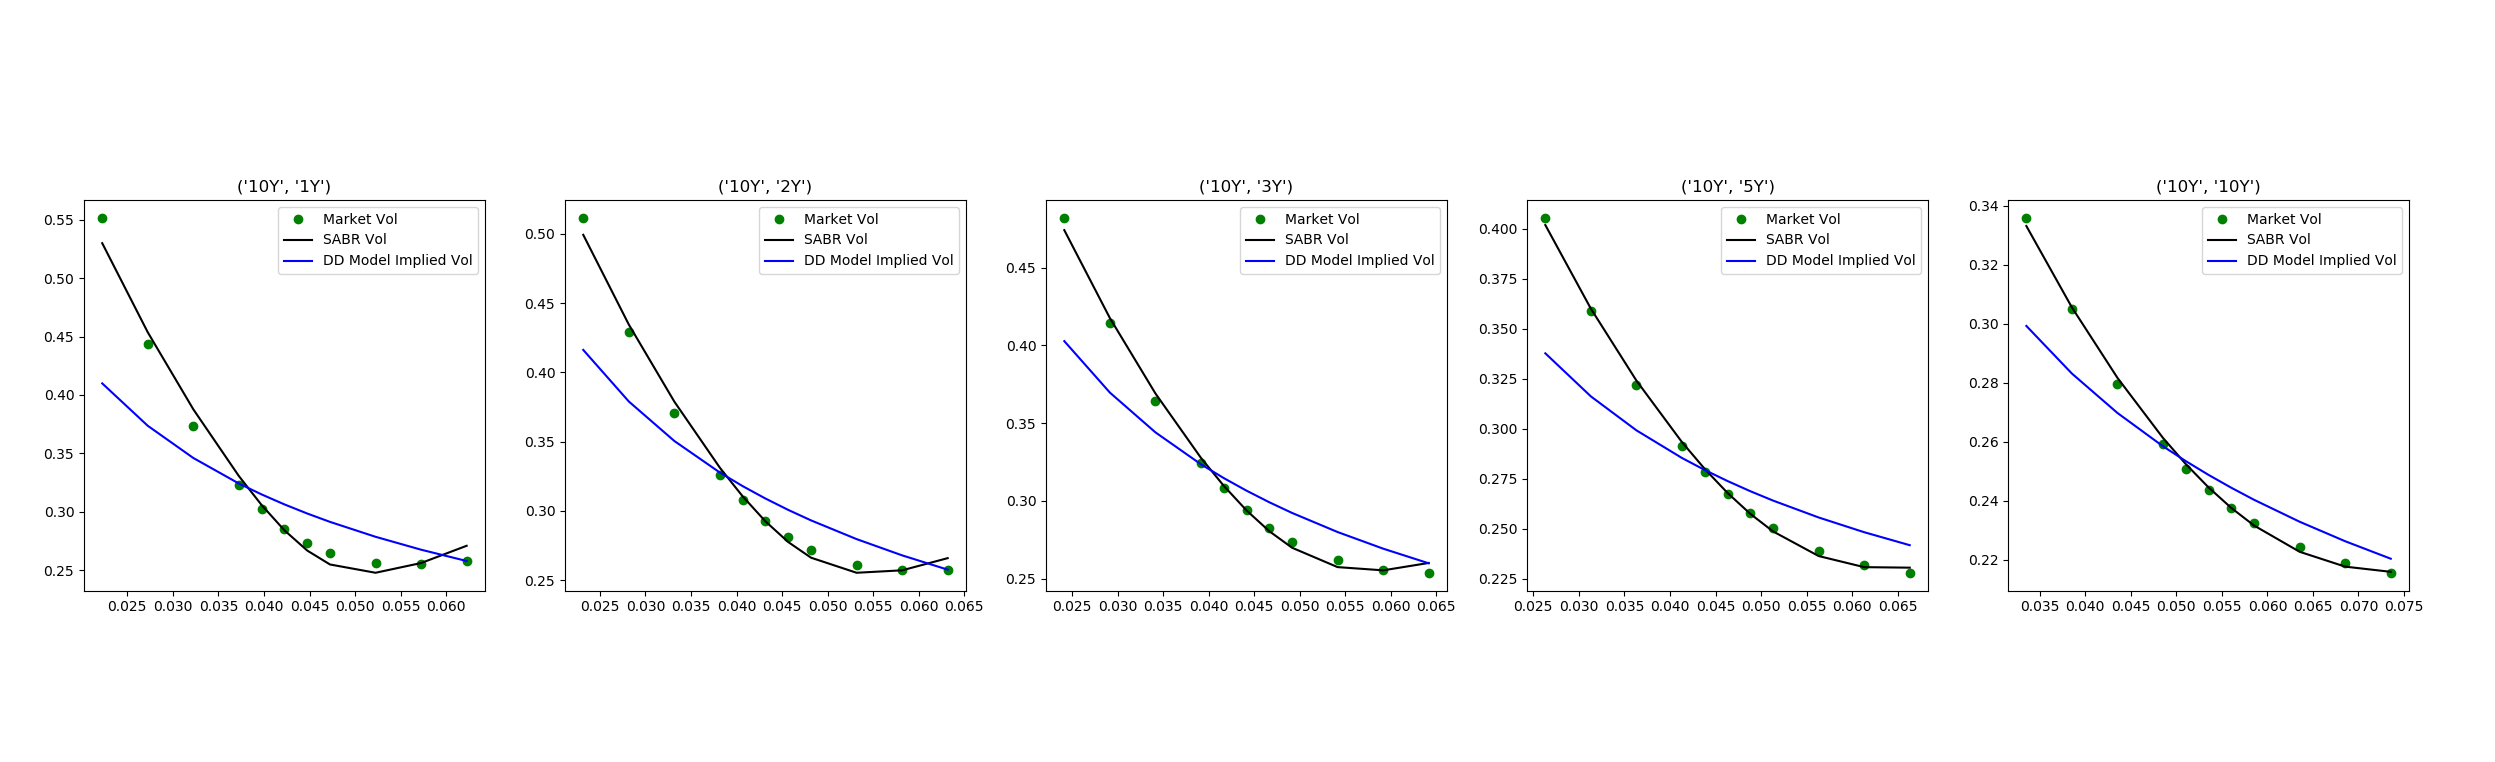
\includegraphics[width=1\linewidth]{./images/10Y.png}
	\caption{10y expiry swaption: Tenor from 1y to 10y}
	\label{fig:sub1}
\end{figure}

bla bla bla bla...

bla bla bla bla...

bla bla bla bla...


\end{document}